
\section{Modeling as Programming}
\label{sec:modeling-as-programming}

In this section we shall attempt to explore the argument that
modeling can be perceived as programming. We will do this through
a small collection of examples, illustrating how what is normally
considered as modeling can be perceived as programming. 
Models are encoded in the Scala programming language, which is
sufficiently high-level to illustrate the point.
We start with class diagrams, as found in UML and SysML, then move on to a classical formal specification language such as \vdmpp{}, and finally discuss DSLs (Domain-Specific Languages).

\subsection{Modeling of Class Diagrams}
\label{sec:complex-classes-in-scala}

A commonly used part of UML and SysML is the class diagram. The class diagram is a visualization of data structures as nodes and edges. Nodes represent data elements and edges represent the relationships between data elements. To take an
example, consider the class diagram in Figure \ref{fig:library}
(the example is adopted from \cite{oclinecoreTutorial}). This diagram models libraries of books. In this diagram a box (node) denotes a type, a set of objects of that type. Hence for example the top node \name{Library} 
(references to text, for example names, in models are enclosed in \name{...}) denotes the type of libraries: a set
of library objects each representing a library.
A library has a name, which is a string. Note that
such data of primitive types (strings, integers, reals, Booleans, ...) are represented as so-called {\em attributes} and are declared inside the boxes instead of as edges, although in principle they can be perceived edges to boxes representing primitive types\footnote{This is an example of a discussion
about semantics that can throw a project meeting off its course.}. 
A library consists of (left arrow) 
a collection of books (zero or more represented by 
the {\em multiplicity} $0 .. *$),
reachable from a library object via the field \name{books}. In the other direction: a book is related to zero or one ($0 .. 1$) libraries.
Similarly, a library (right arrow) has associated a collection of
members. Books and members have names. In addition each book has as
attribute the number of books on shelf. Finally, a loan is a 
connection between a book and a member, and a library has 
associated a collection of (current) loans.

\begin{figure}[ht]
\centering
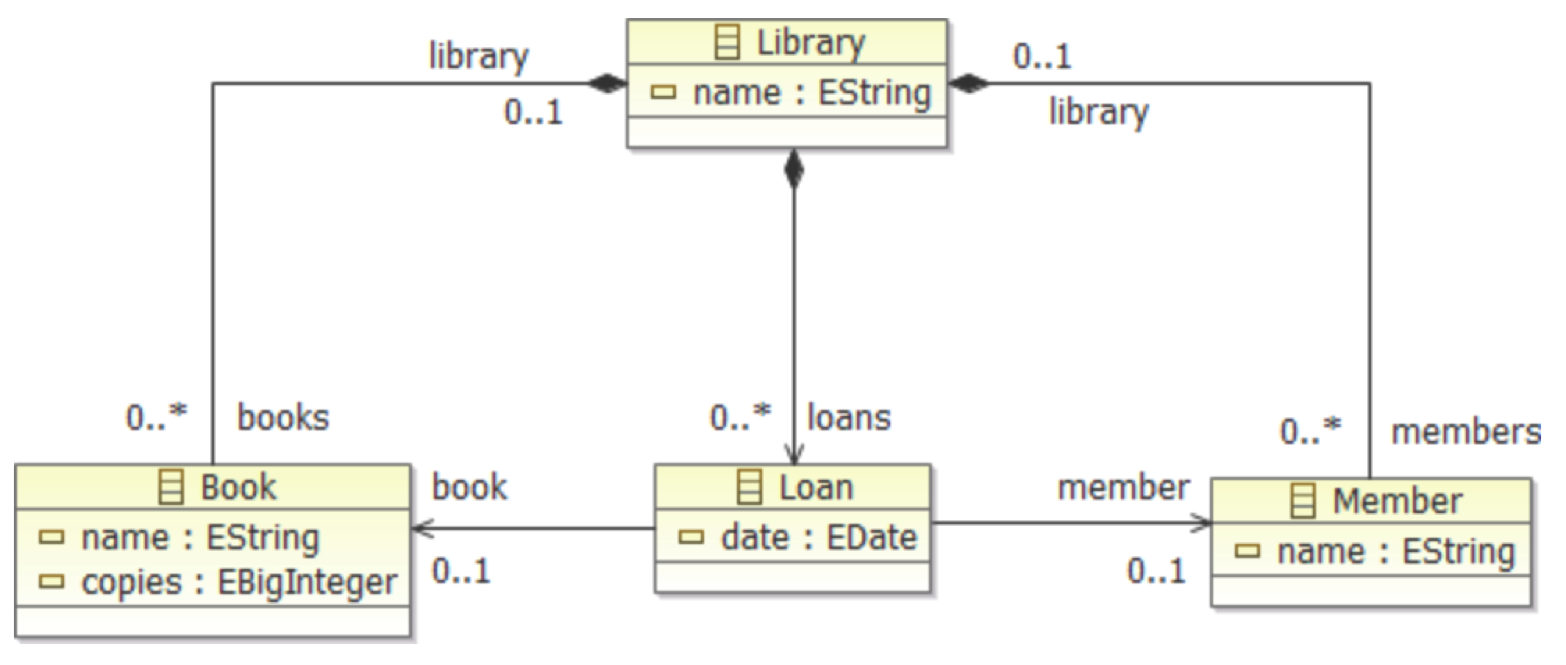
\includegraphics[width=0.9\textwidth]{images/library.png}
\caption{The book library (from \cite{oclinecoreTutorial})}
\label{fig:library}
\end{figure}

\begin{figure}
\begin{schema}{Book}
	name: \seq CHAR \\
	copies: \num
\where
	copies > 0
\end{schema}
\caption{Z model of books in a library}
\label{fig:book-z}
\end{figure}

In many modeling situations such diagrams form the core of the 
modeling effort. Constraints can be added to such diagrams.
For example one constraint could be that the number of copies of a 
book should be positive. Such a 
constraint (not shown) can be added inside a special constraint box on the 
diagram  in Figure \ref{fig:library}, attached to the \name{Book} 
box with a dotted line. It is interesting to note, that a 
box with an associated constraint (written in another box and linked with a line) conceptually is very similar 
to the idea of a Z schema \cite{Spivey-Z-92}, as shown in Figure 
\ref{fig:book-z}\footnote{Note that the constraint can actually be 
avoided in Z by  defining the type of \izlang{copies} to be 
$\mathbb{N}_1$, the natural numbers starting from 1.}.
This schema represents the fundamental concept of a model: a 
signature (the declaration of \izlang{name} and \izlang{copies} above 
the line with their types) and then zero or more axioms (below the 
line). 
%
Attempts have been made to provide textual versions of UML and 
SysML diagrams. An example is  the K specification language 
\cite{havelund-k-modelsward-2016}, that was developed at JPL. 
The expression language of K as well as Z 
(what is written in constraints) is predicate 
logic. Both languages support datatypes such as sets, including 
advanced set expressions such as set comprehension. K is 
object-oriented and is inspired by Z, as well as by
other languages, such as VDM \cite{vdm78,bjoerner-jones-82,jones90,vdmplusplus05} and RAISE \cite{raise92}. 

Another textual notation coming out of the model-based engineering community itself is OCLInEcore \cite{oclinecore}, 
which is an attempt 
to define a textual language combining the structure oriented 
Ecore meta-model
of the Eclipse Modeling Framework (EMF)
\cite{emf} with the 
OCL constraint language (Object Constraint 
Language) 
\cite{ocl}. OCL is a declarative expression language that is now 
part of the UML 
standard. OCL descended from Z, but is based on chained method 
calls read from left to right, starting from {\em finite} 
collections, in contrast to predicate logic. For example OCL does 
not have general universal and existential quantification over 
infinite sets. In predicate 
logic we would write a universal quantification over a set/type 
$S$ as follows: $\forall x : S \bullet P(x)$, meaning: for all $x$ 
in the set $S$, $P(x)$ is true. In OCL one would 
write this as:
\iocl{S->forAll(x | P(x))}. However, OCL requires $S$ to be 
finite,
in contrast to predicate logic, where $S$ can be infinite. This
is the major distinction between OCL and predicate logic, in 
addition to the alternative syntax. OCL is executable, given
a model instance.


%The \name{Book} class with the added constraint can be expressed 
%in K as shown in Figure 
%\ref{fig:book-k}, very similar
%to the Z specification. 

%\begin{figure}
%\begin{center}
%\begin{tabular}{c}
%\begin{lstlisting}[language=klang]
%class Book {
%  name : String
%  copies : Int
%   
%  req copies > 0
%}
%\end{lstlisting}
%\end{tabular}
%\end{center}
%\caption{K model of books in a library}
%\label{fig:book-k}
%\end{figure}

In order to illustrate OCLInEcore we expand our example by adding 
the following requirement: ``{\em The number of loans that a book 
is part of should be less than or equal to the 
number of copies of the book}''. The OCLInEcore model 
in Figure \ref{fig:book-oclinecore} formalizes this requirement.
For this purpose, in addition to the two attributes \iocl{name} and \iocl{copies}, two {\em properties} are defined. 
In contrast to an attribute, 
which has a primitive type, a property is linked to one or 
more objects of another user-defined 
type (those drawn as boxes in class diagrams).
The property \iocl{library} links a book to the library it is part 
of, and is the ``{\em opposite property}'' of the \iocl{books} 
property of the \iocl{Library} (expressed using the \iocl{#}-
notation), meaning that if a book is in the \iocl{books} set (technically 
a bag) of a library, then the library is also in the 
\iocl{library} of the book. The `\iocl{?}' represents 0 or 1.

\begin{figure}
%\begin{center}
%\begin{tabular}{c}
\begin{lstlisting}[language=oclinecore,frame=single,backgroundcolor=\color{light-gray}]
class Book {
  attribute name : String;
  attribute copies : Integer;

  property library#books : Library[?];
     
  property loans : Loan[*] { derived }
  {
    derivation: library.loans->select(book=self);
  }

  operation isAvailable() : Boolean[?]
  {
    body: loans->size() < copies;
  }
     
  invariant CopiesPositive:
    copies > 0;
     
  invariant SufficientCopies:
    loans->size() <= copies;     
}
\end{lstlisting}
%\end{tabular}
%\end{center}
\caption{OCLInEcore model of books in a library (from \cite{oclinecoreTutorial}, modified)}
\label{fig:book-oclinecore}
\end{figure}

The property \iocl{loans} denotes a collection of \iocl{Loan} 
objects and is derived (meaning its value depends on other values), 
with the formula defining 
its value provided as an OCL expression.
The expression reads as follows: from this book (referred to as 
\iocl{self} later in the expression), retrieve the library it is 
part of, retrieve the 
loans of this library, and select those for which the book is 
equal to \iocl{self}. For a given collection \iocl{S}, the 
notation \iocl{S->M(...)} means calling the method \iocl{M} on the 
set \iocl{S}. Hence in this case the
\iocl{select(predicate)} method is defined on sets and returns the 
subset of elements of the set satisfying the predicate.
The two invariants can now be formulated, and their explanation should at this point be straight forward.
The {\em operation} \iocl{isAvailable} is defined to illustrate that one can also define such, here with an OCL expression as body. One can also define operations with side-effects specified with pre/post conditions. No code with side-effects, however, is allowed in 
bodies of operations, which seems to be a limitation, and a sign
of an attempt to move towards a programming language, but not all
the way.

The main point we are trying to make here is that the OCLInEcore 
model, which in reality is very similar to a Z specification 
(signature + axioms), can (for the most part) be elegantly 
expressed in the Scala programming language. This is shown in 
Figure \ref{fig:book-scala}. The class \iscala{Book} extends the
class \iscala{Model}, which we have programmed to offer 
various methods for writing models, including the 
\iscala{invariant} method used to define 
invariants. What in the OCLInEcore model was the property 
\iscala{loans} and the operation \iscala{isAvailable}, are here 
modeled as methods (using the \iscala{def} keyword). 
Multiplicities such as \iocl{Loan[*]} are modeled using Scala's 
collection libraries, in this case \iscala{Set[Loan]}. The Scala 
definitions should be somewhat obvious. It is clear that Scala in 
this case can model this problem in a manner comparable to OCLInEcore. In 
addition, Scala offers so much more than OCLInEcore, such as an 
actual programming language.

\begin{figure}
%\begin{center}
%\begin{tabular}{c}
\begin{lstlisting}[language=scala,frame=single]
trait Book extends Model {
  var name: String
  var copies: Int
  var library: Library

  def loans: Set[Loan] =
    library.loans.filter(_.book eq this)

  def isAvailable(): Boolean =
    loans.size < copies

  invariant("CopiesPositive") {
    copies > 0
  }

  invariant("SufficientCopies") {
    loans.size <= copies
  }
}
\end{lstlisting}
%\end{tabular}
%\end{center}
\caption{Scala program modeling books in a library}
\label{fig:book-scala}
\end{figure}

\begin{figure}[htb]
\begin{center}
\begin{tabular}{c}
\begin{lstlisting}[language=scala]
trait Model {
  type Constraint = Unit => Boolean

  var constraints: List[(String, Constraint)] = Nil

  def invariant(name: String)(c: => Boolean) {
    constraints ::= (name, (Unit => c))
  }

  def verify() {
    for ((n, c) <- constraints) assert(c(), n)
  }
}
\end{lstlisting}
\end{tabular}
\end{center}
\caption{Support for defining invariants in Scala}
\label{fig:invariant-scala}
\end{figure}

The only code that has to be written to provide support for 
writing
class invariants is the definition of the class \iscala{Model}, 
which is shown in Figure \ref{fig:invariant-scala}. Without going 
into details, the class defines a method \iscala{invariant},
which as argument takes a Boolean call-by-name argument. 
The argument is not evaluated before the method body is executed, 
rather, it is only evaluated whenever referred to. In this case
it is stored, still unevaluated, in a list of invariants, all
of which can then be verified on an object of this class 
with a call of \iscala{verify}. Note that such invariants
(specifications) in addition can be the target of more formal analysis, just as they can in a formal specification language.


\subsection{\vdmpp{} Specifications}
\label{sec:vdm-in-scala}

As another example, we shall consider a chemical plant alarm 
management system, first modeled in \vdmpp{} in 
\cite{vdmplusplus05} and also later modeled in Scala in 
\cite{havelund-scala-vdm-12}, which goes into further detail comparing \vdmpp{} and Scala. We show here a slight modification of 
the \vdmpp{} specification as well as the 
corresponding Scala program. In \cite{vdmplusplus05}
the example specification was associated with 
a corresponding UML class diagram to illustrate how the two
techniques can co-exist. Here we shall put emphasis on
\vdmpp{} and its relationship to Scala.

The system shall manage the calling out of experts to deal with 
operational faults discovered in a 
chemical plant. 
Two operations must be provided.
\ivdm{ExpertToPage}: Upon detection of a faulty condition, an 
alarm is raised, and this operation must find an expert on duty 
able to handle the alarm. Each alarm is associated with a specific 
qualification required to fix the causing
problem, and each expert is associated with a set of 
qualifications. Upon an alarm, an expert must be found, and paged, 
that is on duty during the corresponding period and with the right 
qualification.    
\ivdm{ExpertIsOnDuty}: returns the periods during 
which an expert is on duty.      
In addition to providing these two operations, the state of the 
system must satisfy the following
{\em invariant}:
(i) There must be experts on duty during all periods 
allocated in the system. 
(ii) For any alarm and for any period, there should exist an 
expert assigned to that period that has the qualification required
to fix the source problem of the alarm.

The \vdmpp{} class \ivdm{Plant} in Figure \ref{fig:plant-vdm} 
is part of the model of this system (other classes/types shown in
\cite{vdmplusplus05} have been left out here: 
\ivdm{Alarm}, \ivdm{Period}, and \ivdm{Expert}).
The body of this class is divided into three sections: {\em 
instance variables} (mutable variables), {\em functions} (with no 
side-effects), and {\em operations} (with side-effects). An 
invariant defined by the function \ivdm{PlantInv} is imposed on 
the instance variables. The corresponding Scala program modeling the plant is shown in Figure \ref{fig:plant-scala}. We shall not go into the further details, except for mentioning the use of the
\ivdm{suchthat} method in the Scala program, defined in the \ivdm{Model} class, 
which from a finite set selects an element satisfying a predicate provided as argument.

\begin{figure}
%\begin{center}
%\begin{tabular}{c}
\begin{lstlisting}[language=vdm,frame=single,backgroundcolor=\color{light-gray}]
class Plant
  instance variables
    alarms : set of Alarm;
    schedule : map Period to set of Expert;
    
    inv PlantInv(alarms,schedule);

 functions
    PlantInv: set of Alarm * map Period to set of Expert -> bool
    PlantInv(as,sch) ==
      (forall p in set dom sch & sch(p) <> {}) 
        and
      (forall a in set as &
         forall p in set dom sch & 
           exists expert in set sch(p) &
             a.GetReqQuali() in set expert.GetQuali());

  operations
    public ExpertToPage: Alarm * Period ==> Expert
    ExpertToPage(a, p) ==
      let expert in set schedule(p) be st
        a.GetReqQuali() in set expert.GetQuali()
      in
        return expert
    pre a in set alarms and p in set dom schedule
    post let expert = RESULT in
      expert in set schedule(p) and
      a.GetReqQuali() in set expert.GetQuali();
		
		 
    public ExpertIsOnDuty: Expert ==> set of Period
    ExpertIsOnDuty(ex) ==
      return {p | p in set dom schedule & ex in set schedule(p)};
end Plant
\end{lstlisting}
%\end{tabular}
%\end{center}
\caption{\vdmpp{} model of plant}
\label{fig:plant-vdm}
\end{figure}

\begin{figure}
%\begin{center}
%\begin{tabular}{c}
\begin{lstlisting}[language=scala,frame=single]
trait Plant extends Model {
  var alarms: Set[Alarm]
  var schedule: Map[Period, Set[Expert]]

  invariant{PlantInv(alarms, schedule)}

  def PlantInv(alarms: Set[Alarm], schedule: Map[Period, Set[Expert]]): Boolean =
    (schedule.keySet forall {p =>  schedule(p) != Set()}) 
      &&
    (alarms forall { a =>
      schedule.keySet forall { p =>
        schedule(p) exists { expert =>
          a.reqQuali in expert.quali
        }
      }
    })

  def ExpertToPage(a: Alarm, p: Period): Expert = {
    require((a in alarms) && (p in schedule.keySet))
    schedule(p) suchthat { expert =>
      a.reqQuali in expert.quali
    }
  } ensuring { expert =>
    (a.reqQuali in expert.quali) &&
      (expert in schedule(p))
  }

  def ExpertIsOnDuty(ex: Expert): Set[Period] =
    schedule.keySet filter { p => ex in schedule(p) }
}
\end{lstlisting}
%\end{tabular}
%\end{center}
\caption{Scala program modeling plant}
\label{fig:plant-scala}
\end{figure}

\subsection{Domain-Specific Languages}
\label{sec:dsl-in-scala}

We consider the ability to define domain-specific languages (DSLs) 
an essential part of a modeling/programming framework. This form of 
activity is supported 
within the UML/SysML community through meta-modeling and profiles. 
Programming languages have been slower to pick up this concept, 
although an early language such as Lisp supported macros
from its birth. A modern programming language such as Scala 
supports definition of
so-called {\em internal} DSLs with a collection of a few 
elegant language features. In this section we shall illustrate this 
with an example
DSL for monitoring event sequences. 
The example was also listed in \cite{havelund-joshi-experience-2014}.
An {\em internal} DSL is an extension of the programming language, 
in this case 
effectively an API, however, expressed in such a way that use of 
this API
has the flavor of new syntax added to the language.

\begin{figure}
%\begin{center}
%\begin{tabular}{c}
\begin{lstlisting}[language=scala,frame=single]
class NoLockCycles extends Monitor {
  "r1" -- 'acquire('t,'l) |-> 'Locked('t,'l)
  "r2" -- 'Locked('t,'l) & 'release('t,'l) |-> remove('Locked)
  "r3" -- 'Locked('t,'l1) & 'acquire('t,'l2) |-> 'Edge('l1,'l2)
  "r4" -- 'Edge('l1,'l2) & 'Edge('l2,'l3) & not('Edge('l1,'l3)) |-> 'Edge('l1,'l3)
  "r5" -- 'Edge('l1,'l2) |-> { if (get('l1) == get('l2)) fail() }
}
\end{lstlisting}
%\end{tabular}
%\end{center}
\caption{Scala program written in the rule DSL, 
monitoring lock operations}
\label{fig:deadlocks-scala}
\end{figure}

The DSL illustrated here is LogFire \cite{havelund-logfire-sttt14},
created for rule-based programming, and specifically for 
writing temporal trace properties. We shall not go into the details of LogFire (the reader is referred to \cite{havelund-logfire-sttt14}), but only show a model written in this DSL, 
and briefly explain how the DSL is defined. 
A monitor is specified as a set of rules, each of the form: 

\[
  \textit{name}\ \verb+--+\ \textit{condition}_1\ \& \ldots \&\ \textit{condition}_n\ \longmapsto\  \textit{action}
\]

\noindent
A rule consists of a left-hand side: a list of conditions, and a 
right-hand side:
an action. The rules operate on a set of facts, the 
{\em fact memory} (implemented as a Rete network \cite{forgy-rete-82}) 
where conditions check the presence or absence of certain facts, 
and the action adds or deletes 
facts, or executes any Scala code inserted as part of the action. Figure 
\ref{fig:deadlocks-scala} illustrates 
a monitor, which monitors $acquire(thread,lock)$ and 
$release(thread,lock)$ events emitted from an instrumented 
multi-threaded application, that uses locks to protect against
data races. The monitor attempts to determine whether any 
group of threads access locks
in a cyclic manner, which potentially can lead to deadlocks (the classical dining philosopher problem). 
A cycle is detected if for any lock $l$ there is 
an edge from $l$ back to itself.

The class contains five rules. Beyond the monitored events
\iscala{acquire} and \iscala{release}, the monitor adds 
and deletes \iscala{Locked(thread,lock)} facts (the thread holds
the lock), and adds \iscala{Edge(lock1,lock2)} facts, representing
that there is an edge from \iscala{lock1} to \iscala{lock2}, indicating that a thread holds  \iscala{lock1} while acquiring
\iscala{lock2}. The class extends the \iscala{Monitor} class which contains the DSL definitions that allow us to write rules in this manner. Specifically the functions: \iscala{--}, \iscala{&}, \iscala{|->}, \iscala{remove}, and \iscala{fail}. 

The implementation of this DSL relies on Scala's (1) 
allowance for methods having symbol names, such as \iscala{--}
and \iscala{|->}, (2) allowance for method calls of the form 
\iscala{obj.method(arg)} to be written as 
\iscala{obj method arg}, and (3) automated insertion (by 
the compiler) of 
user-defined {\em implicit} 
functions that can lift a value of one type 
to a value of another type in places where the compiler's type 
checker fails to type check an expression. For example part of
the DSL implementation are the definitions shown in Figure
\ref{fig:dsl-scala}.
The implicit function \iscala{liftRuleName} 
gets invoked by the compiler automatically when a string is 
followed by the symbol \iscala{--}. It lifts the string (rule name) to an anonymous object, which provides the method \iscala{--}, which when applied to a condition returns
an \iscala{RuleDef} object, which provides the methods \iscala{&}
and \iscala{|->}. This way method calls can be chained together.

\begin{figure}
\begin{center}
\begin{tabular}{c}
\begin{lstlisting}[language=scala]
implicit def liftRuleName(name: String) = 
  new { 
    def --(c: Condition) = new RuleDef(name, List(c)) 
  }

class RuleDef(name: String, conditions: List[Condition]) { 
  def &(c: Condition) = new RuleDef(name, c :: conditions)

  def |->(stmt: => Unit) { 
    addRule(Rule(name, conditions.reverse, Action((x: Unit) => stmt))) 
  } 
}
\end{lstlisting}
\end{tabular}
\end{center}
\caption{Scala rule DSL implementation}
\label{fig:dsl-scala}
\end{figure}

We do notice, however, some drawbacks of the Scala DSL.
Notice the quoted names: \iscala{'acquire}, \iscala{'Locked}, 
\iscala{'t}, etc. These are Scala symbols (elements of the type 
\iscala{Symbol}). It is not possible in this form of DSL to avoid 
these quotes. Likewise, the name of the rule is a string. 
Furthermore, a monitor in this DSL cannot be type checked without 
actually running the monitor. That is to say, Scala's DSL defining
features are not optimal, although they do make defining internal 
DSLs somewhat easier.
